% METODOLOGIA------------------------------------------------------------------

\chapter{DESENVOLVIMENTO}
\label{chap:metodologia}

\textcolor{red}{TODO: intro}

Este capítulo aborda o desenvolvimento do projeto.

\section{CONCEPÇÃO DO PROJETO}
\label{sec:concepcao}

Com base no projeto arquitetônico e a partir do levantamento das tecnologias disponíveis e viáveis (sobretudo pelo custo e pela difusão no mercado), foram definidos os componentes e técnicas a serem utilizadas no projeto eletrônico, cujo diagrama geral é apresentado na \autoref{fig:diagramageral}.

\begin{figure}[H]
    \centering
    \caption{Diagrama geral do projeto eletrônico}
    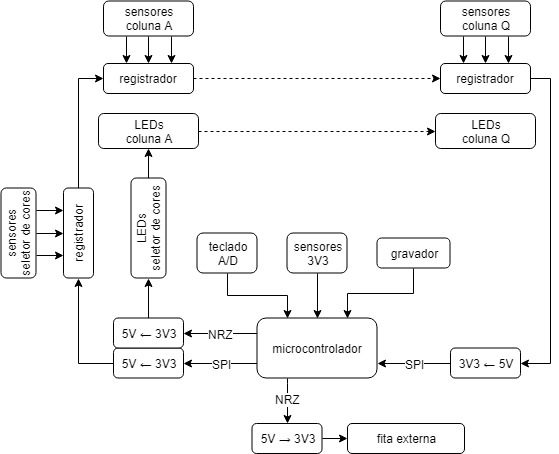
\includegraphics[width=0.8\textwidth]{./dados/figuras/diagrama}
    \fonte{(O AUTOR, 2018)}
    \label{fig:diagramageral}
\end{figure}

A partir do projeto arquitetônico (\autoref{fig:mesa-sup}), que é segmentado em duas partes: Matriz (interação) e Controle (seletor de cores), o projeto eletrônico também foi organizado em 3 subdivisões: Matriz, Interface e Controlador, apresentadas na \autoref{fig:subsecoes}. Dessa forma, pôde-se dar andamento ao projeto por meio de etapas, onde cada fase pode ser considerada um projeto íntegro por si só.

\begin{figure}[H]
    \centering
    \caption{As 3 subseções principais do projeto eletrônico}
    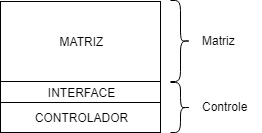
\includegraphics[width=0.40\textwidth]{./dados/figuras/secoes}
    \fonte{(O AUTOR, 2018)}
    \label{fig:subsecoes}
\end{figure}

As subdivisões têm funções bem definidas, apresentadas logo abaixo, e serão discutidas neste mesmo capítulo nos tópicos a seguir.

\begin{itemize}
    \item \textbf{Matriz:} é o setor que pode ser ``pintado com luz'', que contém os LEDs e os sensores de interação. É inteiramente comandada pelo Controlador, através da Interface;
    \item \textbf{Interface:} interliga as subseções Matriz e Controlador: captura e propaga o sinal dos sensores, através dos registradores de deslocamento, e forma a ligação sequencial do barramento dos LEDs;
    \item \textbf{Controlador:} processa todos os LEDs e sensores da mesa. Contém também os LEDs e os sensores do seletor de cores, a parte de processamento, os conversores de nível lógico e os periféricos de gravação e depuração.
\end{itemize}

\textcolor{red}{TODO: especificações, tensão}

\textcolor{red}{TODO: software}

\section{PROJETO DA MATRIZ}
\label{sec:matriz}

O projeto da Matriz foi concebido durante o Programa de Iniciação Científica do qual o autor participou. Nele, o desafio foi o de contemplar todas as 118 bolinhas de \emph{ping-pong} desta seção (e seus respectivos pares sensor-LED), visando robustez e o menor custo.

Para tal, foi definido que a matriz seria arranjada em 17 colunas verticais, conforme apresentado na \autoref{fig:placas-matriz-colunas}. Consequentemente, devido à disposição dos objetos (determinada pelo projeto arquitetônico), essas colunas poderiam conter 5, 6, 7 ou 8 bolinhas e, para abrangê-las da maneira mais proveitosa, as colunas foram combinadas por módulos (placas) de 2 ou 3 bolinhas.

Em geral, as empresas fabricantes de placas de circuito impresso consideram cada modelo de placa como um projeto, devido ao corte do painel, procedimento para os testes elétricos e etc. Assim, se utilizando de apenas 2 modelos de placa, foi possível reduzir o custo do projeto sem dispensar a robustez que as PCIs proporcionam.

\begin{figure}[H]
    \centering
    \caption{Disposição das placas da Matriz}
    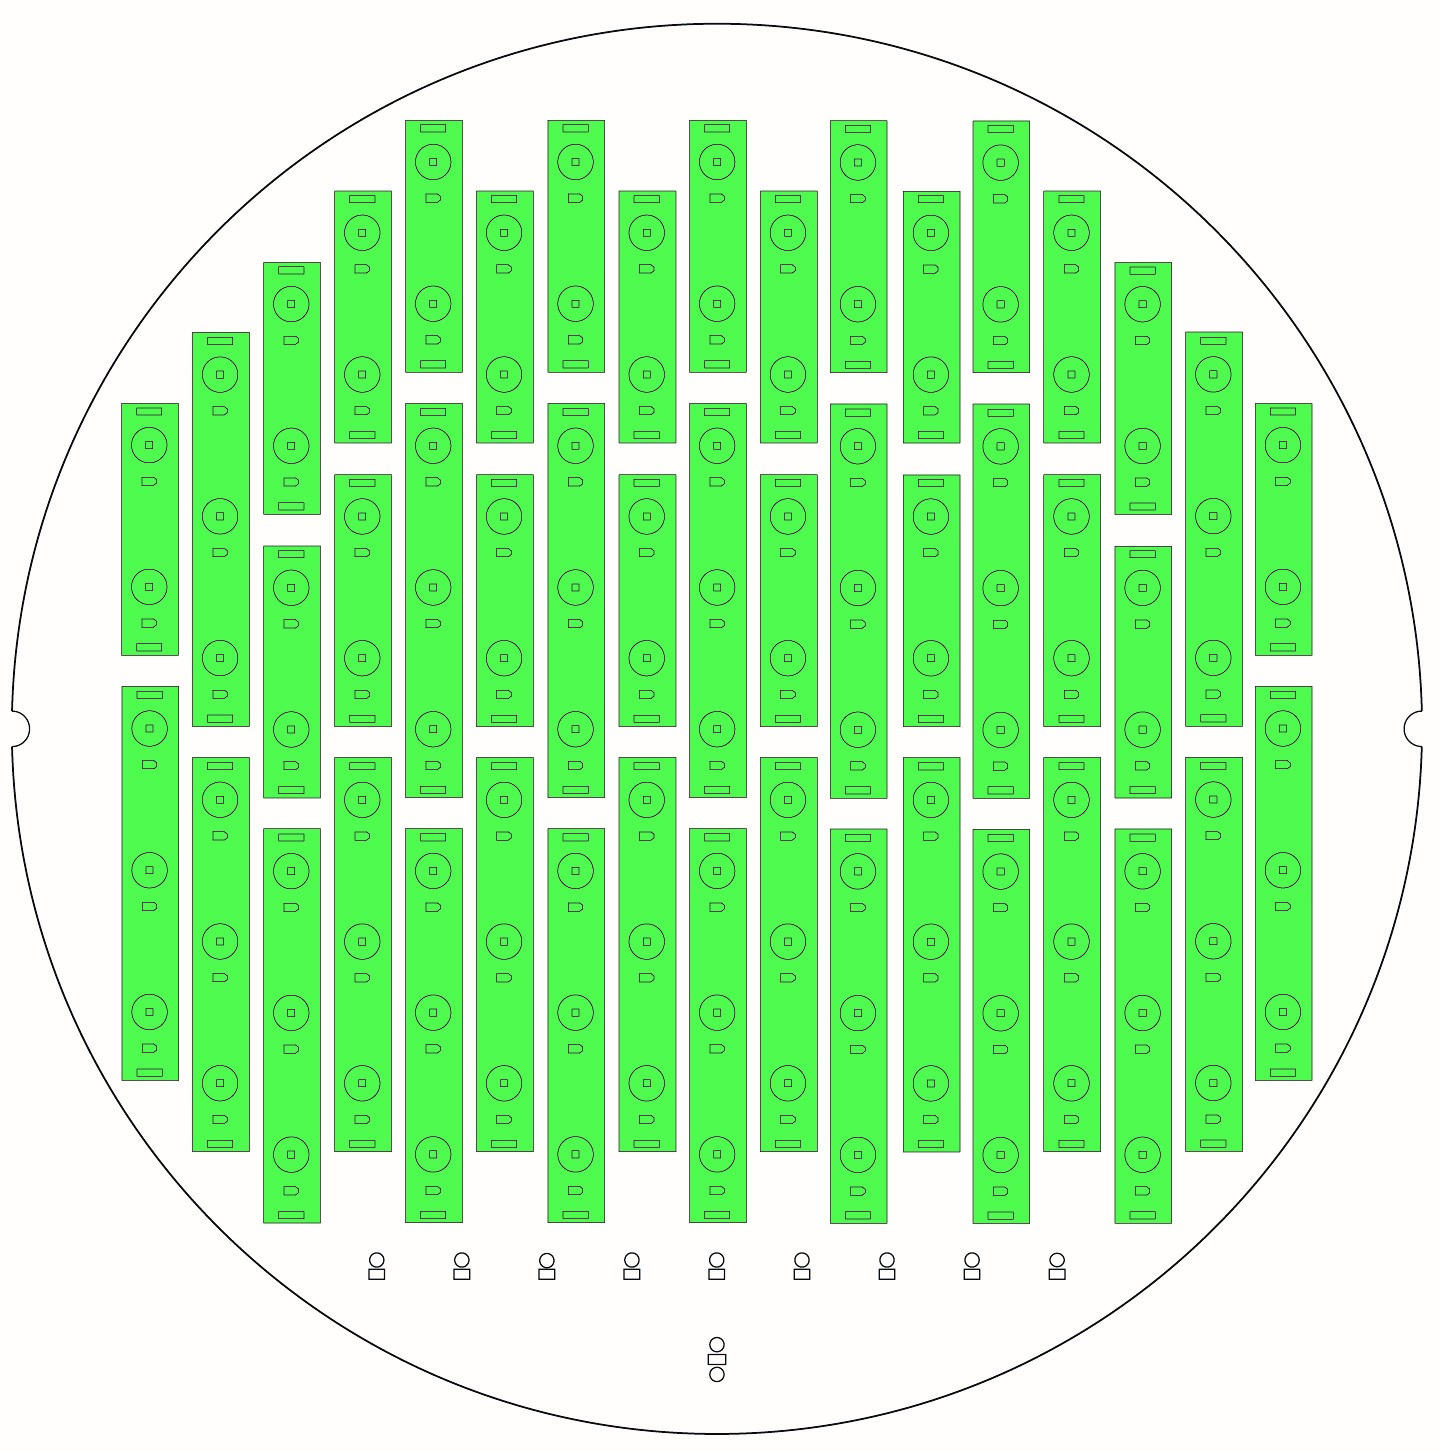
\includegraphics[width=0.7\textwidth]{./dados/figuras/placas-matriz-colunas}
    \fonte{adaptado de (MITSUKO, 2016)}
    \label{fig:placas-matriz-colunas}
\end{figure}

Uma vez definido que a matriz seria composta por placas com 2 ou 3 bolinhas, iniciaram-se os testes de conceito com o protótipo, apresentado na \autoref{fig:matriz-prototipo}. Nesses ensaios, foram testados os conceitos de endereçamento do LED WS2812, a leitura do nível lógico dos sensores através dos registradores de deslocamento e também o modo de conexão entre as placas.

\begin{figure}[H]
    \centering
    \caption{Protótipo das placas da matriz}
    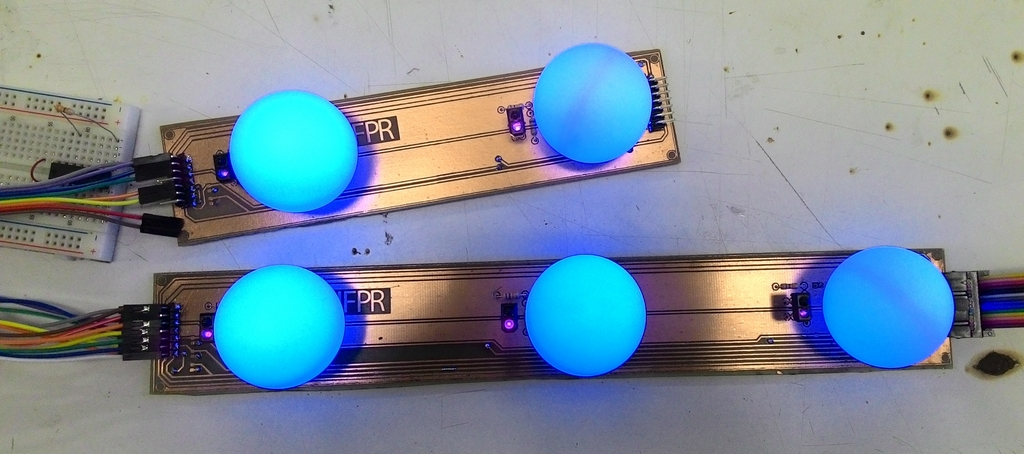
\includegraphics[width=0.8\textwidth]{./dados/figuras/mesa-protoboard}
    \fonte{(O AUTOR, 2017)}
    \label{fig:matriz-prototipo}
\end{figure}

Todos os conceitos propostos foram validados e as 47 placas que compõem a matriz foram confeccionadas em produção industrial. A \autoref{fig:placa2} e a \autoref{fig:placa3} apresentam as faces superior e inferior dos módulos.

\begin{figure}[H]
    \centering
    \caption{Faces da PCI do módulo de 2 bolinhas}
    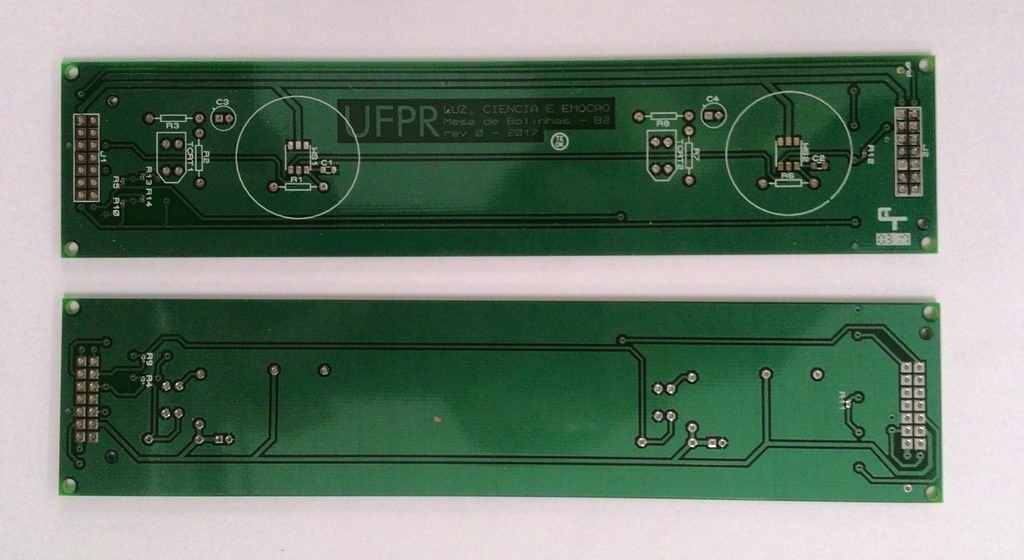
\includegraphics[width=0.8\textwidth]{./dados/figuras/bloco-2}
    \fonte{(O AUTOR, 2017)}
    \label{fig:placa2}
\end{figure}

\begin{figure}[H]
    \centering
    \caption{Faces da PCI do módulo de 3 bolinhas}
    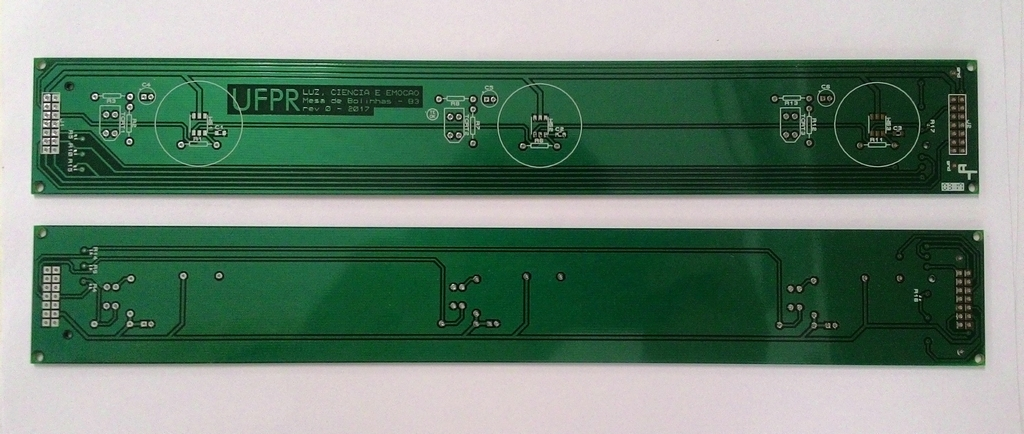
\includegraphics[width=0.99\textwidth]{./dados/figuras/bloco-3}
    \fonte{(O AUTOR, 2017)}
    \label{fig:placa3}
\end{figure}

\textcolor{red}{TODO: o ``resultado da mesa fica nesta seção mesmo?''}

\section{PROJETO DA INTERFACE}
\label{sec:interface}

Como já brevemente introduzido pela \autoref{sec:concepcao} (Concepção do Projeto), a Interface tem a função de interligar as seções Matriz e Controlador. Contudo, deve-se atentar a algumas questões:

\begin{enumerate}[label=\Roman*.]
    \item Tanto o barramento dos sensores, quanto o barramento dos LEDs devem seguir a sequência da esquerda para a direita; de baixo para cima;
    \item Por integrar barramentos de frequências razoáveis - NRZ @800kHz e SPI @4MHz dos LEDs e sensores, respectivamente - deve-se evitar construir trilhas com quinas abruptas, em função da reflexão do sinal;
    %\item As trilhas de potência devem ser adequadas para suportarem a corrente no caso mais extremo.
\end{enumerate}

A questão (I) foi trabalhada visando a redução de custo, decidiu-se que Interface também seria um projeto modular, isto é, esta seção seria dividida em placas do mesmo modelo. Isso é em razão do valor das placas de circuito impresso ser calculado em função de sua área e que cada projeto possui um pedido mínimo. Em outras palavras, quanto maior a área de uma PCI, maior será o seu custo, e quanto mais modelos de placa, maior será a quantidade a ser adquirida, pois cada modelo possui um pedido mínimo para produção. Sendo assim, a Interface foi projetada para abranger todas as colunas da Matriz em duas ``metades'', como é apresentado na \autoref{fig:colunas}. No caso, uma placa teria a função de operar as primeiras 9 colunas (de A a I) e a outra, as 8 colunas restantes (de J a Q).

\begin{figure}[H]
    \centering
    \caption{Divisão das colunas para conexão com a Interface}
    \includegraphics[width=0.7\textwidth]{./dados/figuras/colunas}
    \fonte{adaptado de (MITSUKO, 2016)}
    \label{fig:colunas}
\end{figure}

A \autoref{fig:diagrama-interface} apresenta o diagrama da formação do barramento dos sensores. Nele, cada coluna da Matriz é conectada a um registrador de deslocamento, em forma sequencial (A:1, ..., I:9; J:1, ..., Q:8). Nota-se também que o último registrador da segunda placa não possui conexão, dado que todas as colunas já foram abrangidas registradores precedentes.

\begin{figure}[H]
    \centering
    \caption{Diagrama do barramento da Interface}
    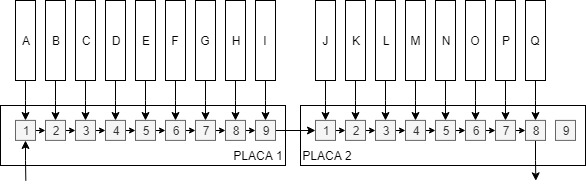
\includegraphics[width=0.75\textwidth]{./dados/figuras/interface}
    \fonte{(O AUTOR, 2018)}
    \label{fig:diagrama-interface}
\end{figure}

Esse direcionamento do barramento é dado por um resistor de $0\Omega$, como apresentado na \autoref{fig:direcionamento-shift} (componente ``R2''). Se montado, o sinal é diretamente conduzido ao conector de saída (``P11''), ignorando o último registrador (``U9'') que, neste caso, não seria montado.

\begin{figure}[H]
    \centering
    \caption{Direcionamento do barramento dos sensores}
    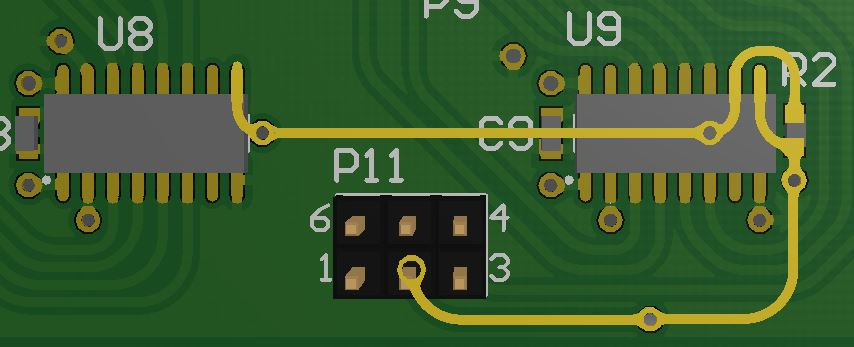
\includegraphics[width=0.6\textwidth]{./dados/figuras/res-dir-shift}
    \fonte{(O AUTOR, 2018)}
    \label{fig:direcionamento-shift}
\end{figure}

De iguais modos, o barramento dos LEDs foi projetado para seguir a mesma sequência (\autoref{fig:sentido-leds}) e o direcionamento entre a última coluna (``P9'') ou o conector de saída (``P11'') também é dado através de um resistor de $0\Omega$ (``R1''), como apresentado na \autoref{fig:direcionamento-leds}.

\begin{figure}[H]
    \centering
    \caption{Sentido do barramento dos LEDs}
    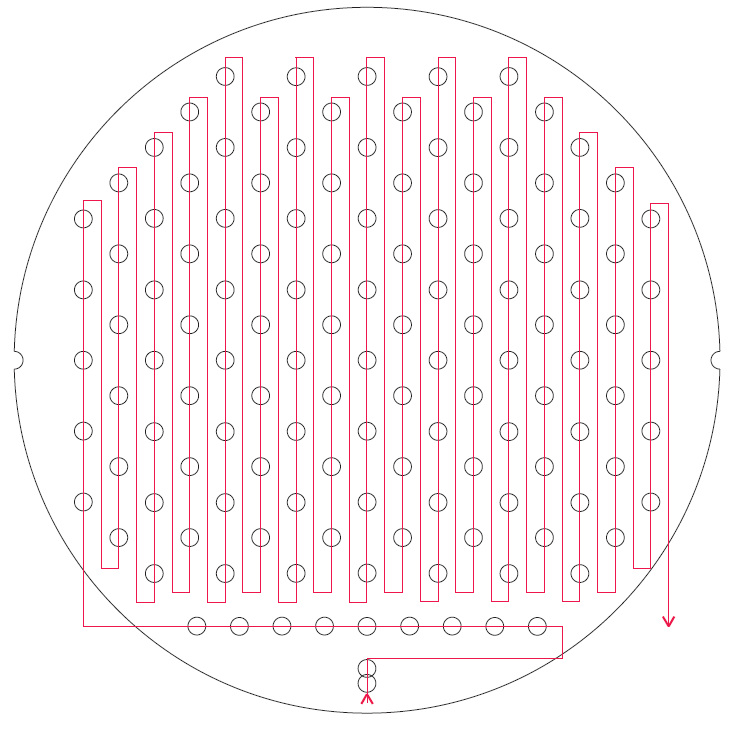
\includegraphics[width=0.75\textwidth]{./dados/figuras/sentido-leds}
    \fonte{adaptado de (MITSUKO, 2016)}
    \label{fig:sentido-leds}
\end{figure}

\begin{figure}[H]
    \centering
    \caption{Direcionamento do barramento dos LEDs}
    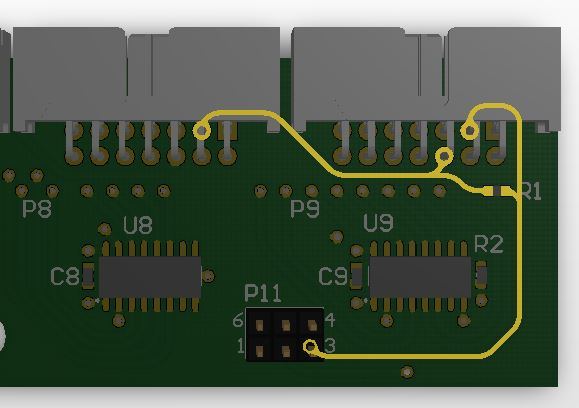
\includegraphics[width=0.6\textwidth]{./dados/figuras/dir-leds}
    \fonte{(O AUTOR, 2018)}
    \label{fig:direcionamento-leds}
\end{figure}

Já em relação à questão (II), sobre a possibilidade de reflexão de sinais devido à perturbação da capacitância e auto-indutância da trilha, seguiu-se a recomendação de leiaute de \cite{datasheet-ti}, apresentada na \autoref{fig:leiaute-ti}.

\begin{figure}[H]
    \centering
    \caption{Recomendação de leiaute para as trilhas de sinal}
    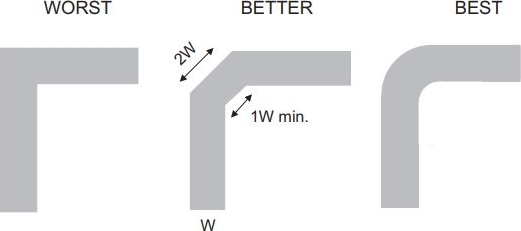
\includegraphics[width=0.5\textwidth]{./dados/figuras/leiaute-ti}
    \fonte{\citeonline{datasheet-ti}}
    \label{fig:leiaute-ti}
\end{figure}

Tal técnica foi aplicada não só nas trilhas de sinais, mas também em todas as ocasiões possíveis, como apresentado na \autoref{fig:trilhas-arredondadas}.

\begin{figure}[H]
    \centering
    \caption{Trilhas arredondadas}
    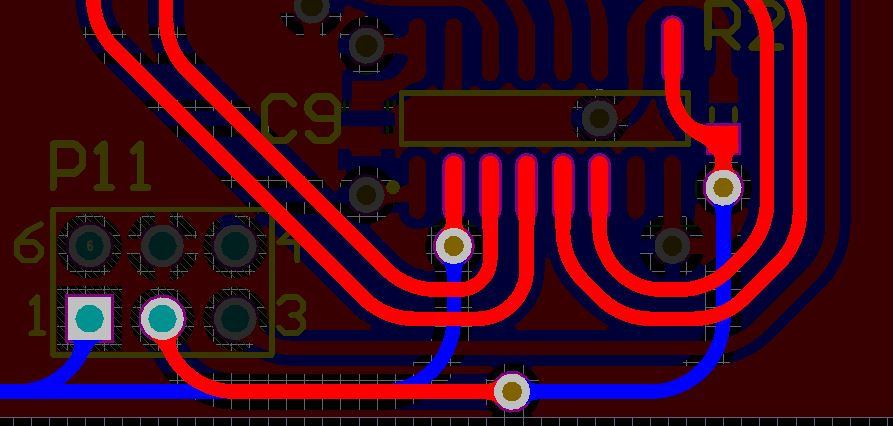
\includegraphics[width=0.7\textwidth]{./dados/figuras/trilhas-arredondadas}
    \fonte{(O AUTOR, 2018)}
    \label{fig:trilhas-arredondadas}
\end{figure}

Além disso, para evitar a propagação do ruído da parte de potência, a alimentação do circuito lógico (``VCC5V'') foi separada da alimentação dos LEDs (``VLED'') e da dos sensores (``VSENSOR''), conforme apresentado na \autoref{fig:interface-alimentacao}. Ademais, a conexão física entre as massas (terra) é feita somente em um único ponto, assim, o retorno da alimentação de potência ("GND\_MATRIX") permanece confinado, não circulando sobre o plano de terra ("GND"). Essa técnica é conhecida por \emph{``net-tie''} e está destacada na \autoref{fig:interface-nettie}.

\begin{figure}[H]
    \centering
    \caption{Separação das alimentações da Interface}
    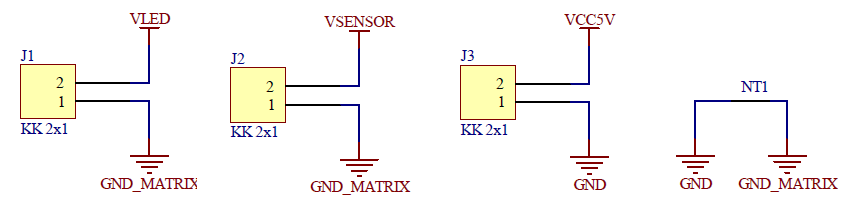
\includegraphics[width=0.85\textwidth]{./dados/figuras/alimentacao-interface}
    \fonte{(O AUTOR, 2018)}
    \label{fig:interface-alimentacao}
\end{figure}

\begin{figure}[H]
    \centering
    \caption{Separação física das massas}
    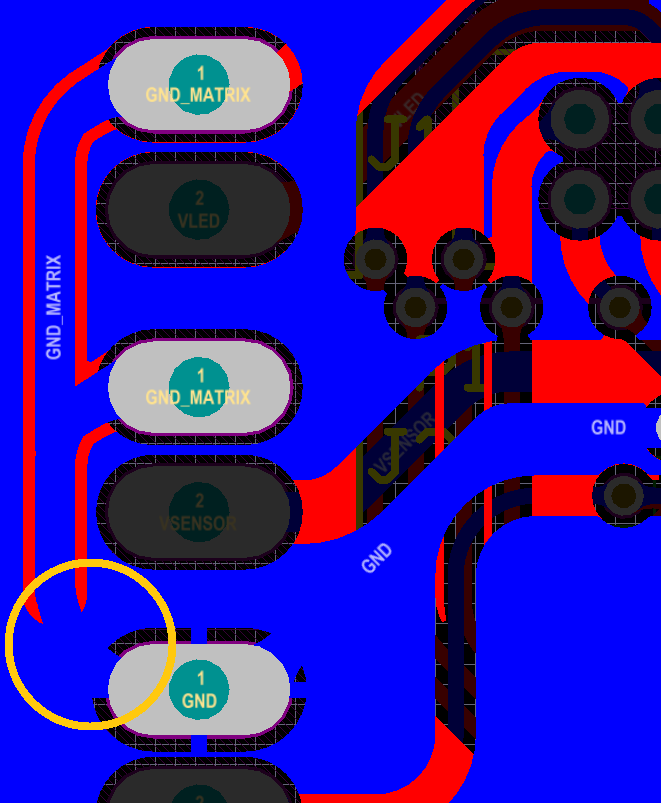
\includegraphics[width=0.4\textwidth]{./dados/figuras/nt-interface}
    \fonte{(O AUTOR, 2018)}
    \label{fig:interface-nettie}
\end{figure}

Por fim, a \autoref{fig:3d-interface} apresenta o modelo 3D da placa de interface. Trata-se de uma PCI face-dupla, 245mm x 32,76mm. Os conectores de alimentação (à esquerda da placa) são da série KK Molex\textsuperscript{\textregistered}, que impedem a inversão de polaridade na conexão com fonte de alimentação externa, e os conectores das colunas (parte superior da placa) são do padrão \emph{Latch-header}, recomendado para aplicações com limitação de espaço. Cada placa suporta até 9 colunas de até 8 sensores, e as PCIs podem ser ligadas em série para compartilharem o mesmo barramento.

\begin{figure}[H]
    \centering
    \caption{Modelo 3D da Interface}
    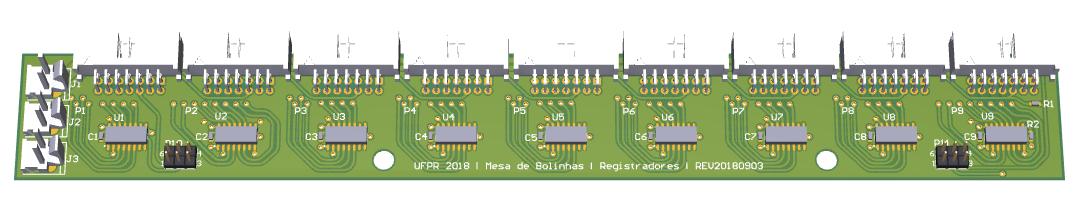
\includegraphics[width=1.0\textwidth]{./dados/figuras/interface-3d}
    \fonte{(O AUTOR, 2018)}
    \label{fig:3d-interface}
\end{figure}

\section{PROJETO DO CONTROLADOR}
\label{sec:controlador}

O Controlador é responsável por comandar os eventos de interação, através da Interface, da seção Matriz. Ademais, engloba também o seletor de cores, circuito de gravação, teclado para depuração e suporte para um barramento externo. A \autoref{fig:diagrama-controlador} apresenta seu diagrama simplificado.

\begin{figure}[H]
    \centering
    \caption{Diagrama da seção Controlador}
    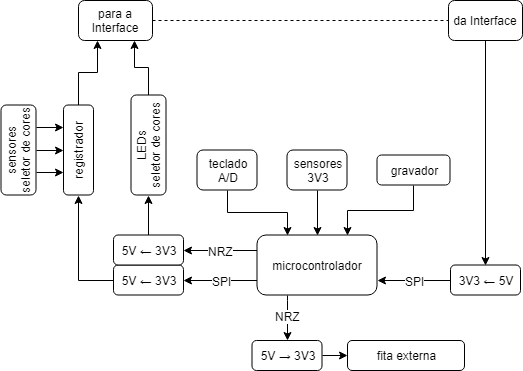
\includegraphics[width=0.75\textwidth]{./dados/figuras/diagrama-controlador}
    \fonte{(O AUTOR, 2018)}
    \label{fig:diagrama-controlador}
\end{figure}

\subsection{ALIMENTAÇÃO  E CONVERSÃO DE NÍVEL LÓGICO}
\label{subsec:alimentacao}

Da mesma forma que na Interface, a alimentação do Controlador também foi dividida, separando os circuitos de potência (``VLED'') e lógico (``VCC5V''), inclusive com \emph{net-tie} isolando fisicamente as massas. Porém, diferente da Matriz, onde a quantidade de LEDs e sensores é muito maior que a do seletor de cores do Controlador, esses circuitos compartilham a mesma alimentação de potência neste projeto. A \autoref{fig:alimentacao-controlador} apresenta o circuito de entrada de alimentação.

Como o microcontrolador operar em 3,3V, houve a necessidade de incluir um regulador para a faixa especificada. Por se tratar de um circuito de carga simples, isto é, de baixo consumo, optou-se por um regulador linear de saída fixa (componente ``U2''). Para protegê-lo da descarga das capacitâncias conectadas à sua saída (por exemplo, o capacitor ``C23''), foi incluído um diodo de \emph{bypass} (``D27'') para desviar a corrente reversa sobre regulador, no caso da fonte externa ser desconectada e a tensão de saída resultar em um potencial mais alto que o de entrada. Esse diodo também possui a função de proteger o regulador caso o desenvolvedor queira alimentar a placa diretamente através do circuito de gravação, a ser discutido mais adiante.

\begin{figure}[H]
    \centering
    \caption{Entrada de alimentação do Controlador}
    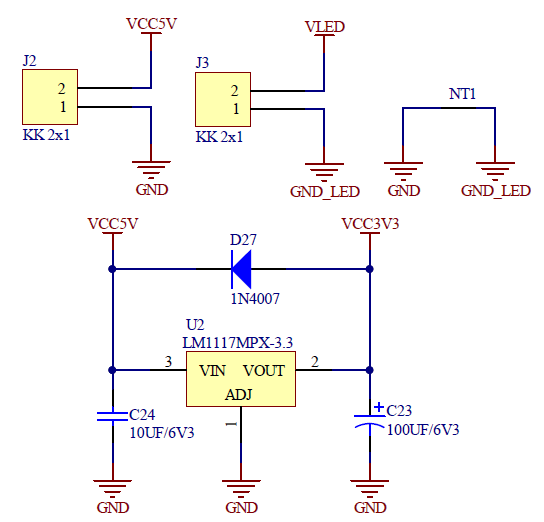
\includegraphics[width=0.7\textwidth]{./dados/figuras/alimentacao-controlador}
    \fonte{(O AUTOR, 2018)}
    \label{fig:alimentacao-controlador}
\end{figure}

\subsection{SELETOR DE CORES}
\label{subse:seletor}

O seletor de cores forma a primeira etapa dos barramentos, seja dos LEDs endereçáveis ou dos registradores de deslocamento. É composto por 10 sensores reflexivos e 11 LEDs endereçáveis, como apresentado na \autoref{fig:seletor-cores}, e a \autoref{fig:diagrama-seletor-cores} apresenta seu diagrama.

\begin{figure}[H]
    \centering
    \caption{Vista do seletor de cores}
    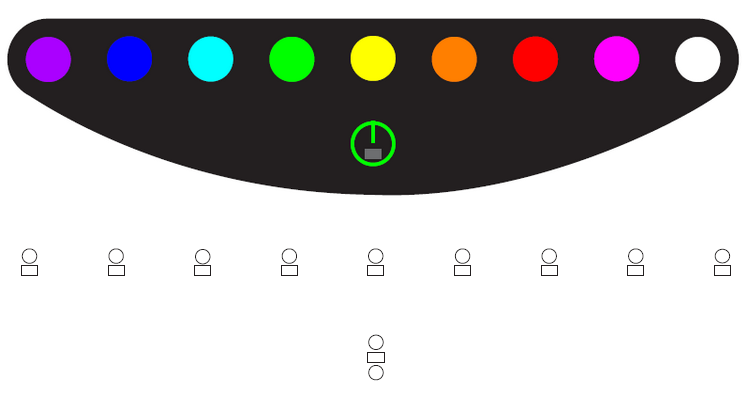
\includegraphics[width=0.75\textwidth]{./dados/figuras/seletor-cores}
    \fonte{adaptado de (MITSUKO, 2016)}
    \label{fig:seletor-cores}
\end{figure}

\begin{figure}[H]
    \centering
    \caption{Vista do seletor de cores}
    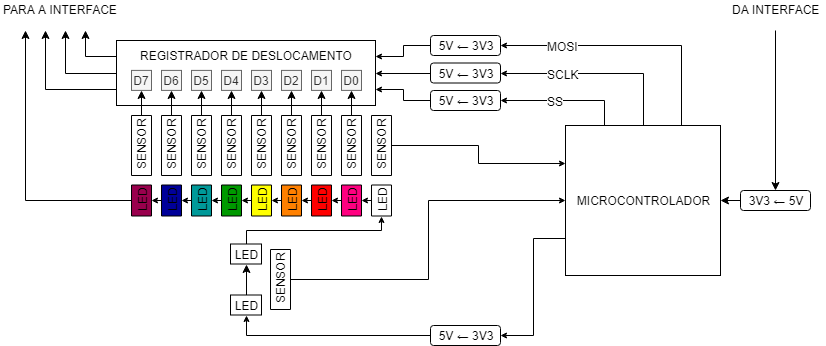
\includegraphics[width=0.99\textwidth]{./dados/figuras/diagrama-seletor-cores}
    \fonte{(O AUTOR, 2018)}
    \label{fig:diagrama-seletor-cores}
\end{figure}

Assim como feito com as colunas da Matriz, por meio das placas da Interface, o registrador de deslocamento é responsável por coletar os níveis lógicos de 8 dos 10 sensores do seletor de cores, restando 2 sensores fora do barramento. Assim, optou-se por conectá-los diretamente aos pinos do microcontrolador, visto que haviam GPIOs livres.

Devido aos LEDs e registradores de deslocamento serem alimentados em 5V, enquanto que o microcontrolador é alimentado em 3,3V, foi necessário adequar os sinais dos barramentos através de conversores de nível lógico. Essa conversão se deu de duas formas, nos seguintes sinais:

\begin{itemize}
    \item De 3,3V para 5V:
        \begin{itemize}
            \item Saída de dados do barramento NRZ (LEDs WS2812)
            \item Saída de dados do barramento SPI (MOSI)
            \item Saída de clock do barramento SPI (SCLK)
            \item Sinal de seleção de periférico do barramento SPI (SS)
        \end{itemize}
    \item De 5V para 3,3V:
        \begin{itemize}
            \item Entrada de dados do barramento SPI (MISO)
        \end{itemize}
\end{itemize}

Os conversores de nível de 3,3V para 5V foram projetados na topologia não-inversora, com transistor NPN operando nas regiões de corte e saturação: mantêm-se base e coletor polarizados - base em 3,3V e coletor em 5V - enquanto que a polarização da junção base-emissor ($V_{BE}$) é dada pela aplicação do sinal no emissor.

A \autoref{fig:3v3-5v} apresenta o esquemático do conversor para o sinal de \emph{clock} do barramento SPI. Nota-se que, quando o sinal ``ESP\_CLOCK'' (saída SCLK do microcontrolador ESP8266) vai a 1-lógico (3,3V), não há diferença de potencial entre a base e o emissor ($V_{BE}=0V$), portanto, o transistor está em corte, logo a saída ``SHIFT\_CLK'' (entrada de \emph{clock} do \emph{shift-register}) vai a 5V (1-lógico).

No caso da aplicação de 0V (0-lógico) por ``ESP\_CLOCK'', a junção base-emissor estará diretamente polarizada, o que, neste caso, levará o transistor à saturação. Com isso, a tensão em ``SHIFT\_CLK'' será a diferença de potencial entre coletor e emissor ($V_{CE}$) somada à queda de tensão sobre o \emph{mosfet} interno da GPIO do microcontrolador, resultando em um potencial relativamente próximo a 0V (0-lógico).

Cabe aqui ressaltar inclusão do diodo de \emph{Baker clamping} para minimizar os efeitos das capacitâncias parasitas do transistor.

\begin{figure}[H]
    \centering
    \caption{Conversor de nível lógico da linha de \emph{clock} do barramento SPI}
    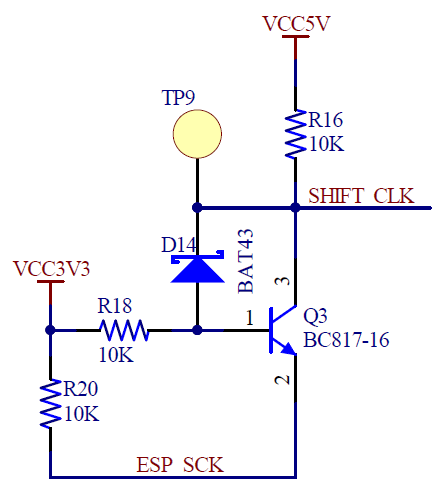
\includegraphics[width=0.4\textwidth]{./dados/figuras/3v3-5v}
    \fonte{(O AUTOR, 2018)}
    \label{fig:3v3-5v}
\end{figure}

Já para a situação de transformação de 5V para 3,3V, como é o caso do retorno do sinal dos registradores de deslocamento das placas de interface (sinal MISO), a implementação do conversor de nível lógico foi dada por um simples divisor resistivo, como apresentado na \autoref{fig:5v-3v3}.

\begin{figure}[H]
    \centering
    \caption{Conversor de nível lógico da linha MISO do barramento SPI}
    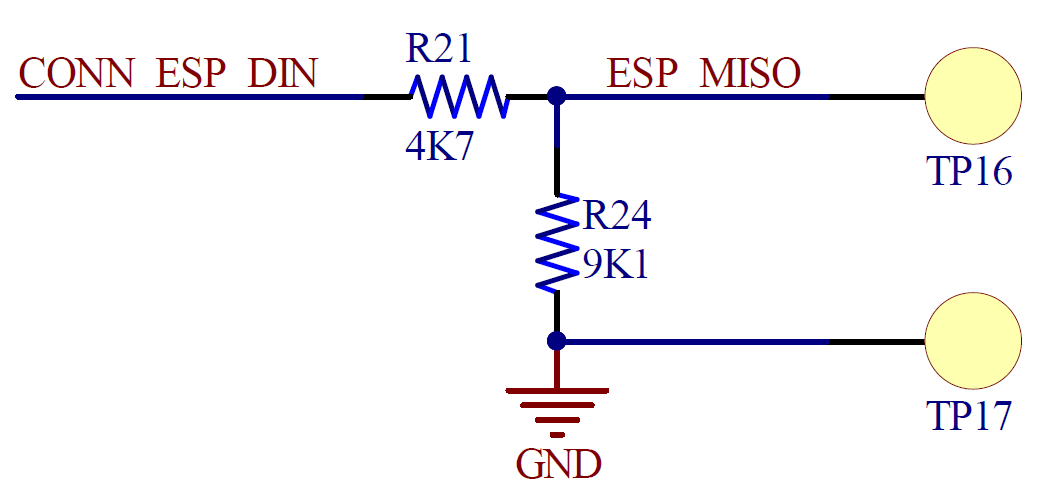
\includegraphics[width=0.5\textwidth]{./dados/figuras/5v-3v3}
    \fonte{(O AUTOR, 2018)}
    \label{fig:5v-3v3}
\end{figure}

Quando aplicado 5V (1-lógico) em ``CONN\_ESP\_DIN'' (entrada de dados do conector, linha MISO do barramento SPI), a tensão em ``ESP\_MISO'' (linha MISO do microcontrolador) será aproximadamente 3,3V (1-lógico), dado pela \autoref{eq:5v-3v3}. De mesmo modo, quando aplicado 0V na entrada do conversor, não haverá queda de tensão sobre o resistor de saída (''`R24``), portanto a tensão em ``ESP\_MISO'' também será 0V (0-lógico).

\begin{equation}
    V = 5V \cdot \frac{9100\Omega}{9100\Omega+4700\Omega} = 3,297V
    \label{eq:5v-3v3}
\end{equation}

\subsection{GRAVADOR}
\label{subsec:gravador}

\textcolor{red}{TODO: comunicação serial}

\textcolor{red}{TODO: botões}

\textcolor{red}{TODO: tabela função XOR? que substitui os botões}

\textcolor{red}{TODO: ftdi}

\subsection{TECLADO ADC}
\label{subsec:tecladoadc}

\subsection{PROJETO DA PCI DO CONTROLADOR}
\label{subsec:pcicontrol}

\textcolor{red}{TODO: 2D PCI controlador}

\textcolor{red}{TODO: NET TIE}

\textcolor{red}{TODO: 3D PCI controlador}

\section{PROJETO DO \emph{FIRMWARE}}
\label{sec:firmware}

\subsection{\emph{DEBOUNCE}}
\label{subsec:debounce}

\subsection{MÁQUINA DE ESTADOS FINITA}
\label{subsec:fsm}

\textcolor{red}{TODO: citar a referencia gang  of 4}

